\chapter{Facial Recognition}\label{ch:face-rec}
Facial recognition is a task of verifying or identifying a person from digital image/video.

As I mentioned in the definition, there are two main subtasks~\cite{FaceRec}:
\begin{enumerate}
    \item \textbf{Verification} deals with verifying whether the person in the image is who he claims he is.
    Typical modern use case of verification is smartphone unlocking with face.
    An example of such system is Face ID developed by Apple Inc.

    \item \textbf{Identification} is a task of matching a person to an identity.
    To formulate it in another way, the goal of identification is to give us an answer to the question of who the person
    in the image is.
\end{enumerate}

\section{Pipeline}\label{sec:pipeline}

Facial recognition pipeline\footnote{A chain of processing elements, arranged so that the output of each element is the
input of the next.} usually has the following four steps:
\begin{enumerate}
    \item The first on is \textbf{face detection} and it deals with determination of face location within the image.
    The output of the algorithm is usually face coordinates and facial landmarks.
    Landmarks are a set of coordinates marking important points of the face (eyebrows, nose, mouth, \ldots).
    The knowledge of these points is a necessity for the following step.
    \item \textbf{Face alignment} is a task of changing the face position in such a way that it resembles the position
    of faces on which the feature extraction model was trained.
    In most of the instances this step improves the accuracy.
    \item \textbf{Feature extraction} is a process of computing a feature vector\footnote{A feature vector is a vector
    that contains information describing an object's important characteristics.} of the face.
    Architecture of models used for feature extraction is described in section~\ref{sec:mod-methods}.
    \item \textbf{Feature matching} uses feature vector from the previous task to identify the person in the image.
    The algorithm uses a database of pre-computed feature vectors and compares them to the newly extracted one.
    The identity associated with the feature vector which has the smallest distance from the extracted one is
    considered to be the identity of the person in the image.
\end{enumerate}

\section{Datasets}\label{sec:datasets}

\subsection{LFW}\label{subsec:lfw}
\subsection{YTF}\label{subsec:ytf}
\subsection{MS-Celeb-1M}\label{subsec:ms1m}

\section{Overview of Modern Methods}\label{sec:mod-methods}
In this section I am about to provide an overview of modern methods/models used for facial recognition.
Models based on CNN architecture~\ref{ch:cnn} achieve state-of-the-art results which is the reason why CNNs dominate the
field of facial recognition and the field of computer vision as a whole now.

Innovations made in the field of computer vision are usually applicable to the subfield of facial recognition as well.
This is manifested in usage of the same model architectures (ResNet~\ref{subsubsec:resnet},
InceptionNet~\ref{subsubsec:inceptionnet}, \ldots) in general image classification as well as in facial recognition.
On the other hand there is a lot of innovation going on in the design of loss functions which work especially well
when used for model training\footnote{Machine learning task of learning a function that maps an input to an output
based on example input-output pairs.} in facial recognition tasks.
This is the reason why this section is divided in two parts: \textit{models}~\ref{subsec:models} and
\textit{loss functions}~\ref{subsec:loss-functions}.

\subsection{Models}\label{subsec:models}
There are two main approaches of training CNNs for face recognition.

The first one is to train a multi-class classifier which can separate identities directly.
An example of such system is DeepFace~\ref{subsubsec:deepface}.

The second approach is to learn embedding using a triplet loss~\ref{subsubsec:triplet-loss} function or similar.
FaceNet~\ref{subsubsec:facenet} is a known example of a system being trained using the second approach.

\subsubsection{DeepFace}\label{subsubsec:deepface}
DeepFace~\cite{DeepFace} is a system developed by FaceBook Inc. in 2014.

The research is notable for its use of advanced alignment technique which consists of three steps:

\begin{enumerate}
    \item The first step is \textbf{2D Alignment} and it begins with detection of 6 fiducial points/landmarks.
    These points and the reference position of points are then used to find a transformation.
    This transformation then generates 2D aligned and cropped image.
    \item The second step is \textbf{3D Alignment}.
    In this step the image is warped onto a generic 3D shape model.
    This is achieved by localization of 67 fiducial points in the image and then fitting an affine
    camera\footnote{linear mathematical model to approximate the perspective projection followed by an ideal
    pinhole camera.} \textit{P} using the generalized least squares solution and the reference position $x_{3d}$ of
    points on the 3D shape model.
    \item \textbf{Frontalization} is the final step and it is achieved by a piece-wise affine transformation T from
    $x_{2d}$ source to $\tilde{x_{3d}}$ target.
    The target $\tilde{x_{3d}}$ is a list of positions of reference fiducial points from previous step enriched with
    residuals \textit{r}.
    These residuals were added to the reference positions $\tilde{x_{3d}}$ to account for non-rigid deformations which
    are not modeled by the affine camera \textit{P}.
    Without these residuals, all faces would be warped into the same shape losing important discriminative factors.
\end{enumerate}

\begin{figure}[H]
    \centering
    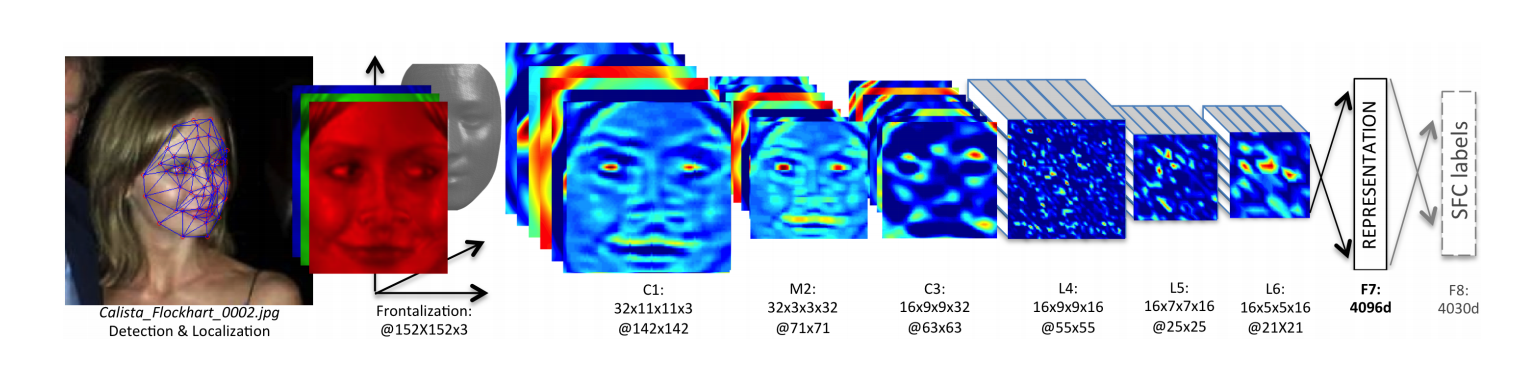
\includegraphics[width=\columnwidth]{images/face-recognition/deepface.png}
    \caption{Outline of DeepFace architecture~\cite{DeepFace}}
    \label{fig:deepface}
\end{figure}

There are 9 layers in the model with over 120 million parameters.
The process of classification is visualized in the picture~\ref{fig:deepface}.
The model was trained on more than 4 million images and as the name of the research paper~\cite{DeepFace} implies, the
results (\textbf{97.35\%} on LFW dataset) almost matched the results of humans (\textbf{97.53\%} on LFW dataset).


\subsubsection{FaceNet}\label{subsubsec:facenet}
FaceNet~\cite{FaceNet} is a system developed by researchers from Google Inc. in 2015.

Interesting innovation of FaceNet lies in the format of its output.
The output of the network is a vector representing a position in an euclidean space (so called embeddings) instead of a
number representing identity.
This approach allows for straight-forward implementation of \textit{verification} and
\textit{identification}~\ref{ch:face-rec}.
Implementation of verification involves thresholding the distance between two embeddings; and identification becomes
k-NN classification problem.

\begin{figure}[H]
    \centering
    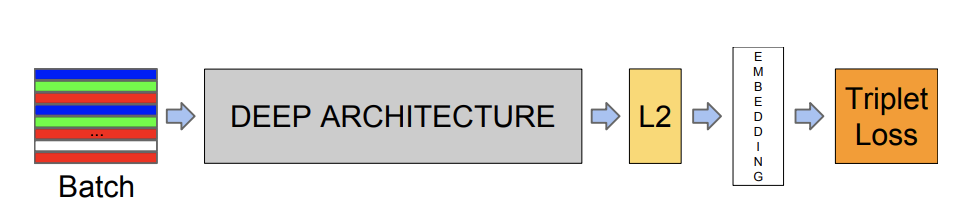
\includegraphics[width=\columnwidth]{images/face-recognition/facenet.png}
    \caption{Outline of FaceNet architecture~\cite{FaceNet}}
    \label{fig:facenet}
\end{figure}

The loss function used to train the model is called \textit{triplet loss}~\ref{subsubsec:triplet-loss}.
Researches at Google came up with new online method\footnote{Training samples are selected during training.} of which
ensures rising difficulty of triplets as the network trains.

The advantages of the model are its accuracy and the compactness of the face representation.
The accuracy of the model exceeded that of human with \textbf{99.63\%} on LFW dataset and the euclidean space has only
128 dimensions.
Another advantage is that the model achieved great results on faces which are not in ideal position without using any
of the complex 3D modeling techniques (as was the case in DeepFace system~\ref{subsubsec:deepface}).
To use proper terms the system is \textit{pose invariant}.

\subsubsection{ResNet}\label{subsubsec:resnet}
A residual neural network (ResNet)~\cite{ResNet} is an ANN which allows for training of networks which contain tens
of layers.
Training of ANN this deep had been practically impossible before the invention of ResNet due to the problem of
\textit{vanishing gradient}\footnote{See footnote on page~\pageref{foot:vangrad}} and \textit{degradation problem}.
The first problem is exposed as a lack of convergence and the second one as a high training error.

Both of these problems have been avoided by implementation of \textit{skip connections} which are illustrated in
figure~\ref{fig:ResNet}.

\begin{figure}[H]
    \centering
    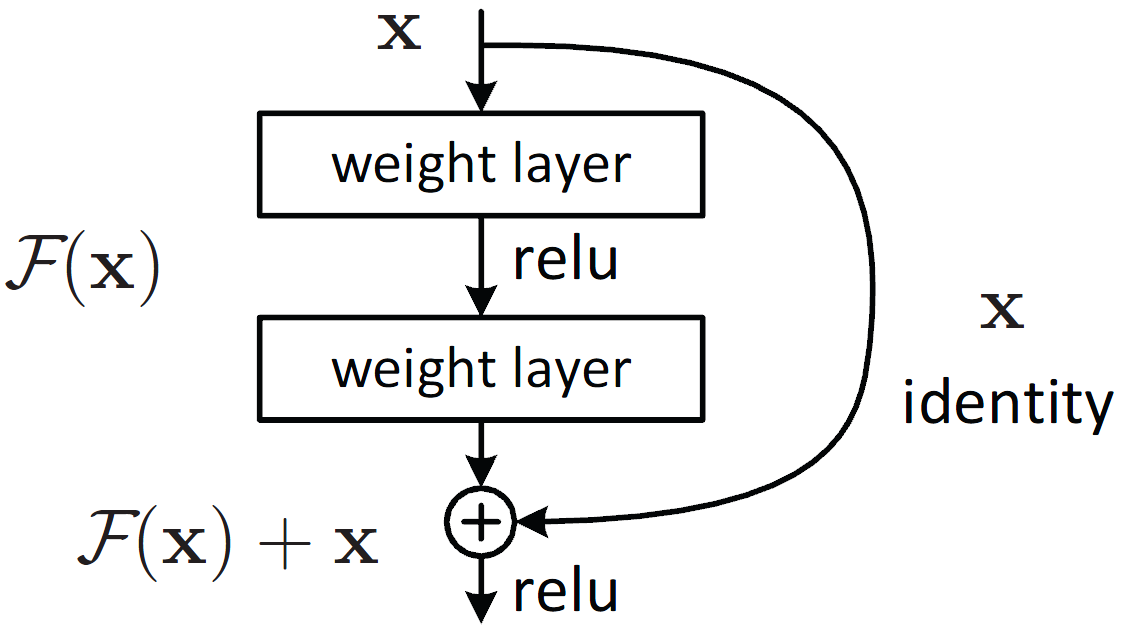
\includegraphics[width=0.9\columnwidth]{images/face-recognition/resnet.png}
    \caption{Residual learning~\cite{ResNet}}
    \label{fig:ResNet}
\end{figure}

The skip connections let the in-between layers fit a residual mapping.
This has proven to be an effective way of using deep neural networks to increase accuracy.

ResNets are widely used in the field of facial recognition as well as in the field of computer vision as a whole.

\subsubsection{InceptionNet}\label{subsubsec:inceptionnet}
InceptionNets are a class of models in which there are multiple kernel sizes operating at the same level.
This is desirable because the right kernel size is dependent on how globally the information is distributed.
A large kernel is preferred when the information is distributed globally and vice versa.

\begin{figure}[H]
    \centering
    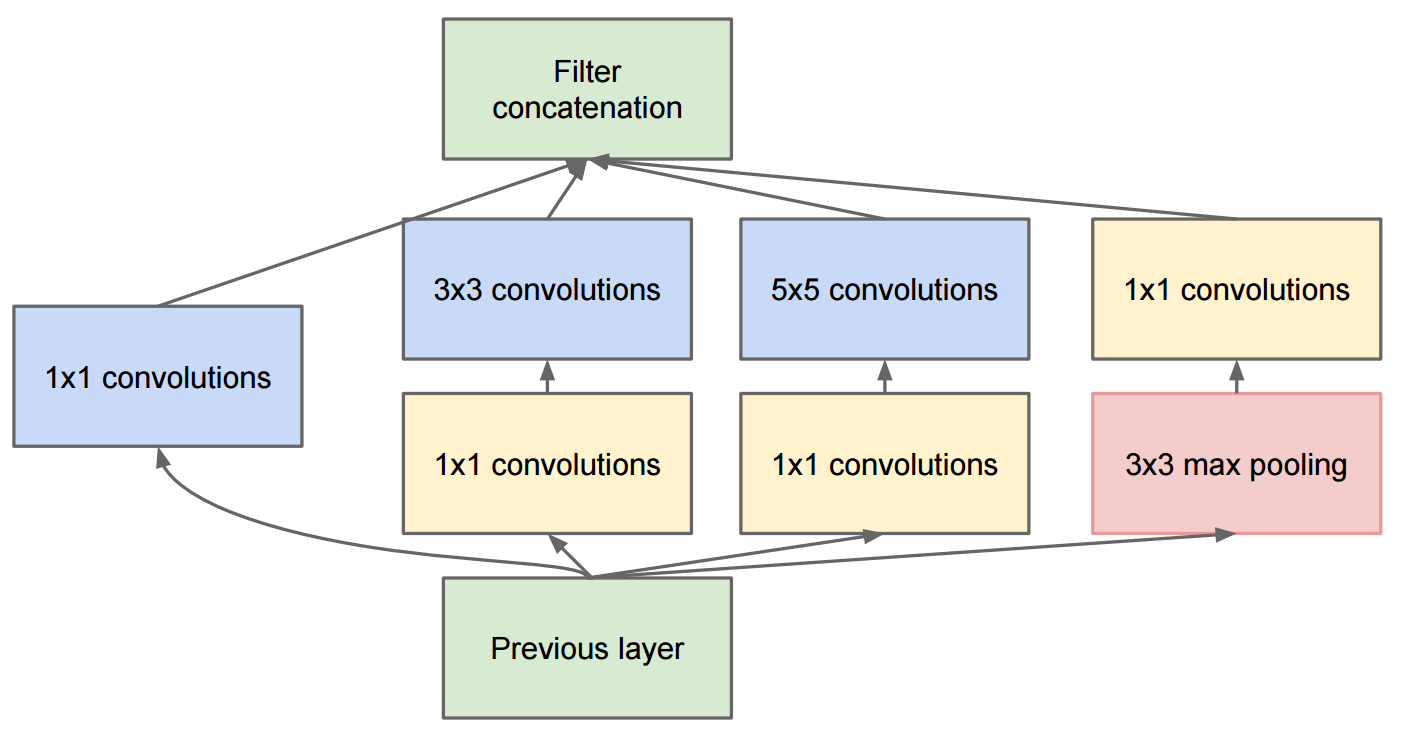
\includegraphics[width=0.9\columnwidth]{images/face-recognition/inceptionnet.png}
    \caption{InceptionNet block~\cite{GoingDeeper}}
    \label{fig:InceptionNet}
\end{figure}

The inception of the inception block (figure~~\ref{fig:InceptionNet}) took place in 2014 in the paper~\cite{GoingDeeper}
published by Google Inc.
Models using inception blocks kept on improving and at the time of writing there is fourth version in use.

\subsubsection{DenseNet}\label{subsubsec:densenet}
DenseNet~\cite{DenseNet} is a type of CNN~\ref{ch:cnn} which was introduced in 2017.
The difference from regular CNNs is that every layer is connected to all the subsequent layers.
Traditional CNN with \textit{L} layers has exactly \textit{L} connections.
On the other hand DenseNet with the same amount of layers contains $\frac{L\left( L+1 \right)}{2}$ connections.
The block of layers is illustrated in figure~\ref{fig:DenseNet}.

\begin{figure}[H]
    \centering
    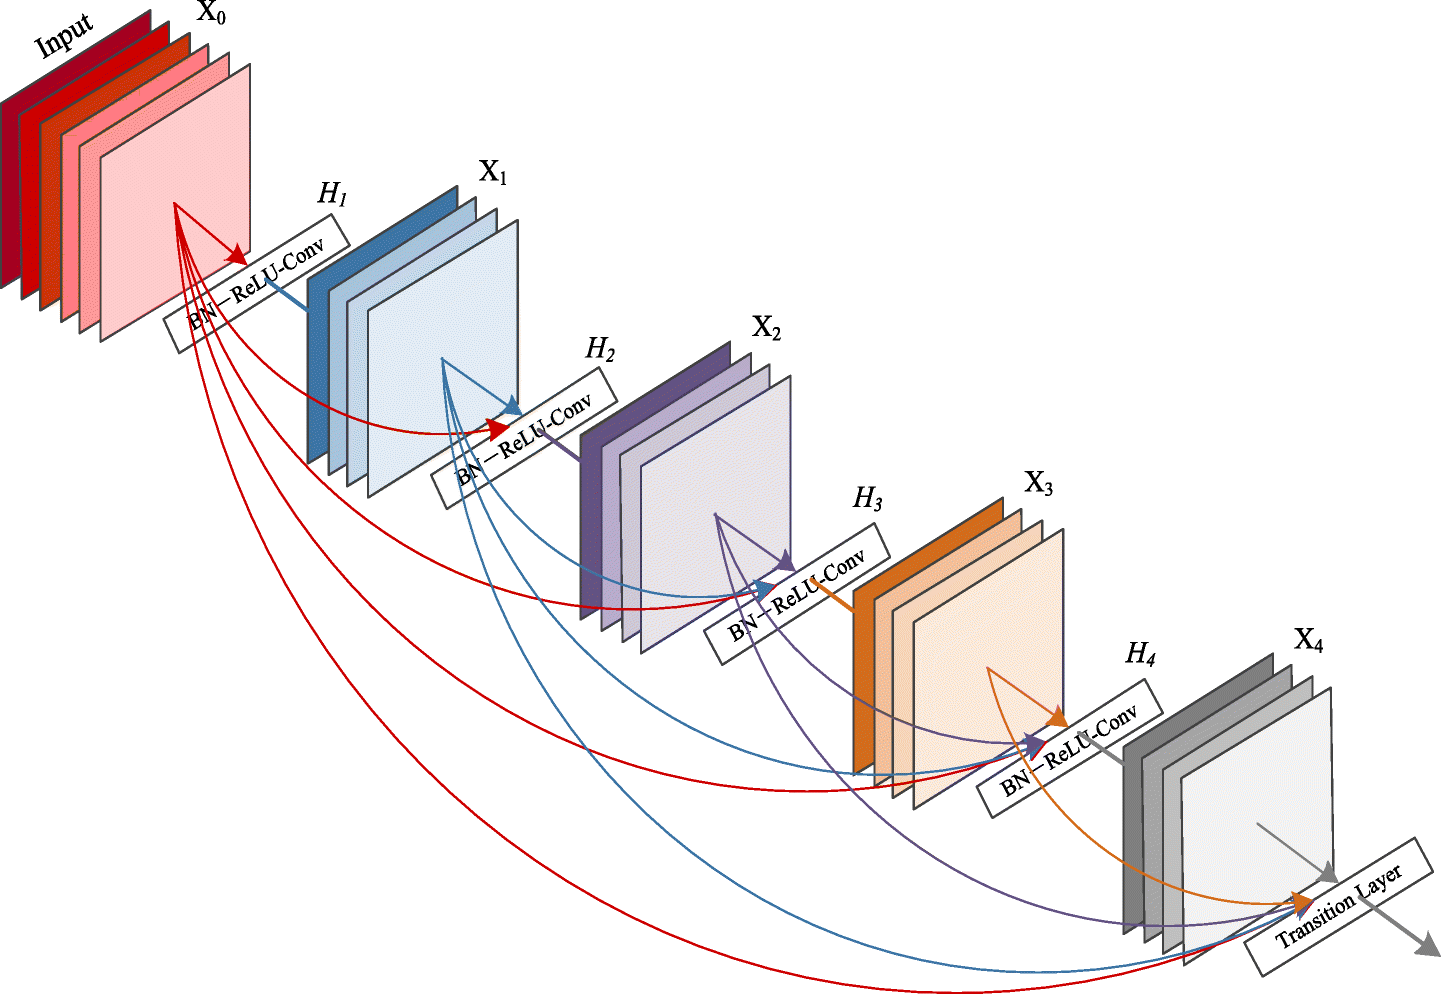
\includegraphics[width=0.9\columnwidth]{images/face-recognition/densenet.png}
    \caption{A 5-layer dense block~\cite{DenseNet}}
    \label{fig:DenseNet}
\end{figure}

DenseNets have several compelling advantages~\cite{DenseNet}.
They alleviate the vanishing-gradient problem, strengthen feature propagation, encourage feature reuse, and
substantially reduce the number of parameters.
\subsection{Loss Functions}\label{subsec:loss-functions}
The main objective of research of loss function is to design a function which leads to a model with superior
discriminative abilities.
How well the model discriminates can be measured by the compactness of clusters and the distance between them.
The goal is for the clusters to be as compact as possible while maximizing the distance in-between them.

\subsubsection{Softmax Loss}\label{subsubsec:softmax-loss}
Softmax~\cite{ArcFace} is the most widely used loss function in general classification tasks and its definition is as
follows:
\begin{equation}
    \label{eq:softmax}
    \mathcal{L}_S = -\frac{1}{N} \sum_{i=1}^{N} \log \frac{e^{W^T_{y_i} x_{i} + b_{y_i}}}
    {\sum_{j-1}^{n} e^{W^T_{j} x_{i} + b_{j}}},
\end{equation}
where $x_i \in \mathbb{R}^{d}$ denotes the feature vector of the \textit{i}-th sample belonging to the $y_i$-th class.
$W_j \in \mathbb{R}^{d}$ is the \textit{j}-th column of the weight matrix $W \in \mathbb{R}^{d \times n}$ and \textit{b}
is the corresponding bias term.
\textit{N} is the batch size and \textit{n} is the class number.

Major drawback of softmax loss is that it doesn't encourage cluster compactness.
In other words, it fails to guarantee similarity among samples within a category.
This makes the learned features not discriminative enough for the open-set face recognition
problem~\footnote{Identifying samples which were not present in the training dataset.}.

The second issue is that the dimension of the output weight matrix grows linearly with the number of identities in the
training set.
This is impractical for large scale deployment.

\subsubsection{Triplet Loss}\label{subsubsec:triplet-loss}
Triplet loss~\cite{TripletLoss} is a loss function which can be optimized by minimizing the distance between
\textit{anchor} and \textit{positive} point while maximizing the distance between \textit{anchor} and \textit{negative}
point.
These points are represented by feature vectors.
The learning process is illustrated in the figure~\ref{fig:tripletloss}.

\begin{figure}[H]
    \centering
    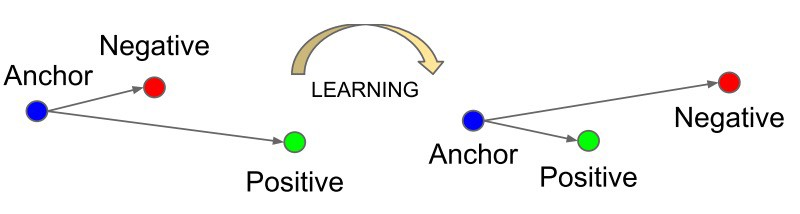
\includegraphics[width=\columnwidth]{images/face-recognition/tripletloss.jpeg}
    \caption{Illustration of the triplet loss~\cite{TripletLoss}}
    \label{fig:tripletloss}
\end{figure}

Anchor and positive points are vectors which belong to the same class whereas negative point belongs to another one.
In the context of facial recognition one class is one identity therefore anchor and positive point are vectorised
representation of two images of one face.

In mathematical terms the loss can be described using Euclidean distance function as follows
\begin{equation}
    \sum_{i}^{N} \left[ \norm{f(x_{i}^{a}) - f(x_{i}^{p}))}^2_2
    - \norm{f(x_{i}^{a}) - f(x_{i}^{n}))}^2_2 + \alpha \right],
\end{equation}
where $f(x_{i}^{a})$, $f(x_{i}^{p})$ and $f(x_{i}^{n})$ are feature vectors of anchor, positive and
negative point of triplet denoted by \textit{i}.
\textit{N} is the number of triplets in the dataset.

The drawbacks of \textit{triplet loss} are the demands entailed by the construction of the triplets.
The number of those is subject to combinatorial explosion and inevitably results in slow convergence and instability
This is a serious issue especially for large datasets.

\subsubsection{Center Loss}\label{subsubsec:center-loss}
The main objective of the research~\cite{CenterLoss} was to design a loss function which solves the main drawbacks of
\textit{sofmax loss}~\ref{subsubsec:softmax-loss} and \textit{triplet loss}~\ref{subsubsec:triplet-loss}.

The discriminative power of the learned features is enhanced by incorporation of the distance of features to the
corresponding class centers.
In other words, the network is penalized whenever the features are too far from the class center.
In the course of training the the centers are updated and the distances of features from centers are minimized.
The model is trained under a joint supervision of softmax loss and center loss.
The effect of these two losses is balanced by a hyperparameter\footnote{A parameter which is not a subject to the
learning process}.
This joint supervision results in a loss function which combines the best of both worlds:
inter-class discriminative power of \textit{softmax loss} and intra-class distance minimization of \textit{center loss}.

The center loss function is intuitively defined by the following equation:
\begin{equation}
    \label{eq:center}
    \mathcal{L}_C = \frac{1}{2} \sum_{i=1}^{m} \norm{x_i - c_{y_i}}_2^2,
\end{equation}
where $c_{y_i} \in \mathbb{R}^{d}$ denotes the $y_i$-th class center of the features.
Recomputing the centers by taking the average of the features over the whole training set id too inefficient and
impractical.

To address this problem the authors proposed updating the centers based on a mini-batch instead of the whole training
set.
To avoid large perturbations caused by mislabeled samples, there is a parameter $\alpha$ with which we control the
learning rate of the centers.

In the equation~\ref{eq:centup} we can see how the center update is computed:
\begin{align}
    \frac{\partial \mathcal{L}_C}{\partial x_i} &= x_i - c_{y_i} \\
    \Delta c_j &= \frac{\sum_{i=1}^m \delta(y_i=j) \cdot (c_j-x_i)}{1+\sum_{i=1}^m \delta(y_i=j)}, \label{eq:centup}
\end{align}
where $\delta(condition)$ is $1$ if the condition is satisfied and $0$ otherwise.

The final loss is described by the following formula:
\begin{equation}
    \label{eq:centerloss}
    \mathcal{L} = \mathcal{L}_S + \mathcal{L}_C = -\sum_{i=1}^{m} \log \frac{e^{W^T_{y_i} x_{i} + b_{y_i}}}
    {\sum_{j-1}^{n} e^{W^T_{j} x_{i} + b_{j}}} + \frac{\lambda}{2} \sum_{i=1}^{m} \norm{x_i - c_{y_i}}_2^2,
\end{equation}

Figure~\ref{fig:centerlosslambda} is a great visualization of the effect of hyperparameter $\alpha$ upon the cluster
compactness.
As is to be expected, higher values of the parameter result in more compact clusters.

\begin{figure}[H]
    \centering
    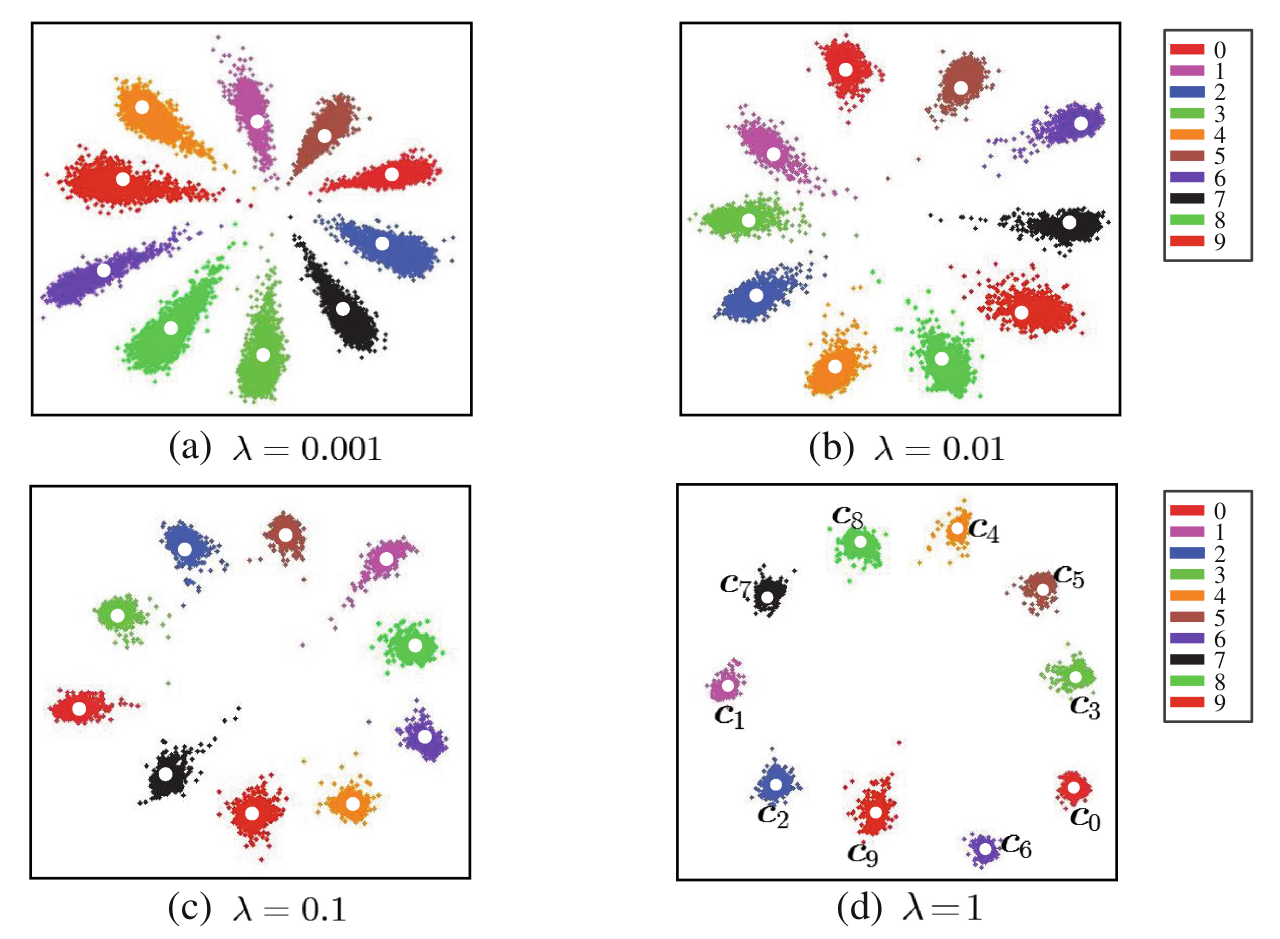
\includegraphics[width=\columnwidth]{images/face-recognition/centerlosslambda.png}
    \caption{Distribution of the features for different values of hyperparameter $\lambda$~\cite{CenterLoss}.
    The white dots $(c_0,c_1,\dots,c_9)$ denote 10 class centers.}
    \label{fig:centerlosslambda}
\end{figure}

\subsubsection{Congenerous Cosine Loss}\label{subsubsec:coco-loss}
Congenerous Cosine Loss~\cite{CocoLoss} (known as COCO loss) is a loss function which was published in 2017.

To define the loss we first have to clarify how the centroid of class \textit{k} is computed.
The centroid\footnote{Center of cluster.} equation is as follows
\begin{equation}
    \boldsymbol{c}_{k} = \frac{\sum_{i \in \beta} \delta \left( l_i, k \right)\boldsymbol{f}^{(i)}}
    {\sum_{i \in \beta} \delta \left( l_i, k \right) + \epsilon} \in \mathbb{R}^{D \times 1},
\end{equation}
where $\beta$ is a mini-batch, $D$ is the feature space dimension, $\delta$ is indicator function, $\epsilon$ is a
trivial number for computation stability, $\boldsymbol{f}^{(i)}$ is the \textit{i}-th feature vector and $l_i$ is
its label.

Now that we have the centroid equation we can define the term we are trying to maximize during model fitting:
\begin{equation}
    p_{l_i}^{(i)} = \frac{exp C(\boldsymbol{f}^{(i)}, \boldsymbol{c}_{l_{i}})}
    {\sum_{k \neq l} exp C(\boldsymbol{f}^{(i)}, \boldsymbol{c}_{k})} \in \mathbb{R},
\end{equation}
where $C$ is standard cosine similarity.

Now we can move on to the final COCO loss function definition:
\begin{equation}
    - \sum_{i \in \beta} \log \left( p_{l_i}^{(i)} \right).
\end{equation}

\subsubsection{SphereFace Loss}\label{subsubsec:sphereface-loss}
SphereFace~\cite{SphereFace} is a loss function which was published in 2018.
The research significantly distinguishes itself from the previously mentioned losses by not relying on euclidean margin.
SphereFace uses angular margin instead.
This has proven to be highly effective in face recognition tasks.

SphereFace loss originates from the softmax loss~\ref{subsubsec:softmax-loss} and its name was inspired by the fact
that the features are projected onto a hypersphere manifold.

To derive SphereFace loss from softmax loss we first incorporate the angle into the softmax equation using the dot
product definition ($a \cdot b = \norm{a} \norm{b} \cos \theta$):

\begin{align*}
    \mathcal{L}_S &= -\frac{1}{N} \sum_{i=1}^{N} \log \frac{e^{W^T_{y_i} x_{i} + b_{y_i}}}
    {\sum_{j-1}^{n} e^{W^T_{j} x_{i} + b_{j}}} \\
    &= -\frac{1}{N} \sum_{i=1}^{N} \log \frac{e^{\norm{W_{y_i}} \norm{x_i} \cos(\theta_{y_i,i}) + b_{y_i}}}
    {\sum_{j-1}^{n} e^{\norm{W_j} \norm{x_{i}} \cos(\theta_{j,i}) + b_{j}}},
\end{align*}
where $\theta_{j,i}$ is the angle between vector $W_j$ and $x_i$.
The meanings of the remaining symbols are equal to those in the softmax equation~\ref{eq:softmax}.


Next we normalize $\norm{W_j} = 1, \forall j$ and set the bias term to 0.
\begin{equation}
    \label{eq:softmaxmod}
    \mathcal{L}_{modified} = -\frac{1}{N} \sum_{i=1}^{N} \log \frac{e^{\norm{x_i} \cos(\theta_{y_i,i})}}
    {\sum_{j-1}^{n} e^{\norm{x_{i}} \cos(\theta_{j,i})}}
\end{equation}
While it's possible to learn features with the modified loss the features are not discriminative enough.
To improve the discriminative power angular margin was incorporated:
\begin{equation}
    \label{eq:ang}
    \mathcal{L}_{ang} = -\frac{1}{N} \sum_{i=1}^{N} \log \frac{e^{\norm{x_i} \cos(m\theta_{y_i,i})}}
    {e^{\norm{x_i} \cos(m\theta_{y_i,i})} + \sum_{j \neq y_i} e^{\norm{x_{i}} \cos(\theta_{j,i})}},
\end{equation}
where $\theta_{y_i,i}$ lies in $\left[ 0, \frac{\pi}{m} \right]$.

The decision boundary for a binary case is defined by:
\begin{equation}
    \label{eq:spherebound}
    \cos{m\theta_1} = \cos{\theta_2},
\end{equation}
where $\theta_i$ is the angle between the feature and weight of class $i$.

To make the loss~\ref{eq:ang} optimizable for CNNs the definition range of $\cos(\theta_{y_i},i)$ is expanded.
This is achieved by replacing the cosine term with monotonically decreasing angle function $\Psi(\theta_{y_i},i)$
\begin{equation}
    \mathcal{L}_{ang} = -\frac{1}{N} \sum_{i=1}^{N} \log \frac{e^{\norm{x_i} \Psi(m\theta_{y_i,i})}}
    {e^{\norm{x_i} \Psi(m\theta_{y_i,i})} + \sum_{j \neq y_i} e^{\norm{x_{i}} \Psi(\theta_{j,i})}}
\end{equation}
The angle function has the following definition:
\begin{equation}
    \Psi(\theta_{y_i,i}) = (-1)^{k} \cos(\theta_{y_{i},i}) -2k,
\end{equation}
where $k \in \left[ 0, m-1 \right]$.
Parameter $m \geq 1$ gives us the control over the angular margin size.

\subsubsection{CosFace Loss}\label{subsubsec:cosface}
CosFace~\cite{CosFace} is another loss using margin to achieve better discriminative power than
softmax~\ref{subsubsec:softmax-loss}.

The decision boundary for binary case is defined by the following equation:
\begin{equation}
    \label{eq:cosbounary}
    \cos{\theta_1} - m = \cos{\theta_2},
\end{equation}
where the symbols have exactly the same meaning as in the equation~\ref{eq:spherebound} of SphereFace decision boundary.
The advantage of CosFace over SphereFace is the ease of optimization.
The reason for that is that the decision boundary of CosFace is not being defined over the angular space.
Optimization in angular space is more difficult because of the non-monotonicity of the cosine function.

Another innovation over SphereFace is that not only is the weight vector $W_j$ normalized, but the feature vectors
$x_i$ as well.
This achieves much lower intra-class variability by concentrating more on the angle during training.
By fixing $\norm{x}$ as some predetermined radius $s$ in equation~\ref{eq:softmaxmod} we get:
\begin{equation}
    \mathcal{L}_{ns} = -\frac{1}{N} \sum_{i=1}^{N} \log \frac{e^{s \cos(\theta_{y_i,i})}}
    {\sum_{j-1}^{n} e^{s \cos(\theta_{j,i})}}
\end{equation}
This loss is called Normalized Softmax Loss (NSL) in the CosFace research paper.
NSL emphasizes correct classification but is not discriminative enough for face recognition tasks.
For this reason (as was mentioned in the SphereFace research as well) the margin is incorporated:
\begin{equation}
    \label{eq:cosface}
    \mathcal{L}_{lmc} = -\frac{1}{N} \sum_{i=1}^{N} \log \frac{e^{s \left( \cos(\theta_{y_i,i}) - m \right)}}
    {e^{s\ \left( \cos(\theta_{y_i,i}) - m \right)} + \sum_{j \neq y_i}^n e^{s\ \cos(\theta_{j,i})}},
\end{equation}
subject to
\begin{align}
    W &= \frac{W*}{\norm{W*}}, \\
    x &= \frac{x*}{\norm{x*}}, \\
    \cos(\theta_j, i) &= W_{j}^T x_i.
\end{align}
The meaning of the equation constituents is equivalent to those in the previous sections.

The equation~\ref{eq:cosface} is the final form of the CosFace loss.
The authors of the research call it the Large Margin Cosine Loss (LMCL).

\subsubsection{ArcFace Loss}\label{subsubsec:arcface}
ArcFace loss is used in this thesis which makes it the topic of the following chapter~\ref{ch:arcface}.